\section{GtkFontDialogButton and
Gsettings}\label{gtkfontdialogbutton-and-gsettings}

\subsection{The preference dialog}\label{the-preference-dialog}

If the user clicks on the preference menu, a preference dialog appears.

\begin{figure}
\centering
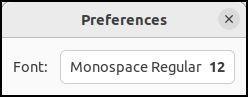
\includegraphics[width=4cm,height=1.6cm]{../image/pref_dialog.png}
\caption{Preference dialog}
\end{figure}

It has only one button, which is a GtkFontDialogButton widget. You can
add more widgets on the dialog but this simple dialog isn't so bad for
the first example program.

If the button is clicked, a FontDialog appears like this.

\begin{figure}
\centering
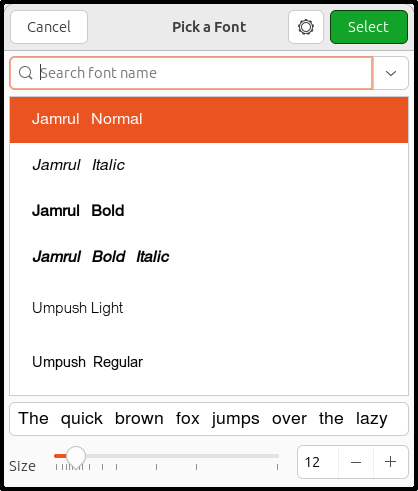
\includegraphics[width=6.27cm,height=7.38cm]{../image/fontdialog.png}
\caption{Font dialog}
\end{figure}

If the user chooses a font and clicks on the select button, the font is
changed.

GtkFontDialogButton and GtkFontDialog are available since GTK version
4.10. They replace GtkFontButton and GtkFontChooserDialog, which are
deprecated since 4.10.

\subsection{A composite widget}\label{a-composite-widget}

The preference dialog has GtkBox, GtkLabel and GtkFontButton in it and
is defined as a composite widget. The following is the template ui file
for TfePref.

\begin{lstlisting}[language=XML, numbers=left]
<?xml version="1.0" encoding="UTF-8"?>
<interface>
  <template class="TfePref" parent="GtkWindow">
    <property name="title">Preferences</property>
    <property name="resizable">FALSE</property>
    <property name="modal">TRUE</property>
    <child>
      <object class="GtkBox">
        <property name="orientation">GTK_ORIENTATION_HORIZONTAL</property>
        <property name="spacing">12</property>
        <property name="halign">GTK_ALIGN_CENTER</property>
        <property name="margin-start">12</property>
        <property name="margin-end">12</property>
        <property name="margin-top">12</property>
        <property name="margin-bottom">12</property>
        <child>
          <object class="GtkLabel">
            <property name="label">Font:</property>
            <property name="xalign">1</property>
          </object>
        </child>
        <child>
          <object class="GtkFontDialogButton" id="font_dialog_btn">
            <property name="dialog">
              <object class="GtkFontDialog"/>
            </property>
          </object>
        </child>
      </object>
    </child>
  </template>
</interface>
\end{lstlisting}

\begin{itemize}
\tightlist
\item
  Template tag specifies a composite widget. The class attribute
  specifies the class name, which is ``TfePref''. The parent attribute
  is \passthrough{\lstinline!GtkWindow!}. Therefore.
  \passthrough{\lstinline!TfePref!} is a child class of
  \passthrough{\lstinline!GtkWindow!}. A parent attribute is optional
  but it is recommended to write it explicitly. You can make TfePref as
  a child of \passthrough{\lstinline!GtkDialog!}, but
  \passthrough{\lstinline!GtkDialog!} is deprecated since version 4.10.
\item
  There are three properties, title, resizable and modal.
\item
  TfePref has a child widget GtkBox which is horizontal. The box has two
  children GtkLabel and GtkFontDialogButton.
\end{itemize}

\subsection{The header file}\label{the-header-file}

The file \passthrough{\lstinline!tfepref.h!} defines types and declares
a public function.

\begin{lstlisting}[language=C, numbers=left]
#pragma once

#include <gtk/gtk.h>

#define TFE_TYPE_PREF tfe_pref_get_type ()
G_DECLARE_FINAL_TYPE (TfePref, tfe_pref, TFE, PREF, GtkWindow)

GtkWidget *
tfe_pref_new (void);
\end{lstlisting}

\begin{itemize}
\tightlist
\item
  5: Defines the type \passthrough{\lstinline!TFE\_TYPE\_PREF!}, which
  is a macro replaced by
  \passthrough{\lstinline!tfe\_pref\_get\_type ()!}.
\item
  6: The macro \passthrough{\lstinline!G\_DECLAER\_FINAL\_TYPE!} expands
  to:

  \begin{itemize}
  \tightlist
  \item
    The function \passthrough{\lstinline!tfe\_pref\_get\_type ()!} is
    declared.
  \item
    TfePrep type is defined as a typedef of
    \passthrough{\lstinline!struct \_TfePrep!}.
  \item
    TfePrepClass type is defined as a typedef of
    \passthrough{\lstinline!struct \{GtkWindowClass *parent;\}!}.
  \item
    Two functions \passthrough{\lstinline!TFE\_PREF ()!} and
    \passthrough{\lstinline!TFE\_IS\_PREF ()!} is defined.
  \end{itemize}
\item
  8-9:The function \passthrough{\lstinline!tfe\_pref\_new!} is declared.
  It creates a new TfePref instance.
\end{itemize}

\subsection{The C file for composite
widget}\label{the-c-file-for-composite-widget}

The following codes are extracted from the file
\passthrough{\lstinline!tfepref.c!}.

\begin{lstlisting}[language=C]
#include <gtk/gtk.h>
#include "tfepref.h"

struct _TfePref
{
  GtkWindow parent;
  GtkFontDialogButton *font_dialog_btn;
};

G_DEFINE_FINAL_TYPE (TfePref, tfe_pref, GTK_TYPE_WINDOW);

static void
tfe_pref_dispose (GObject *gobject) {
  TfePref *pref = TFE_PREF (gobject);
  gtk_widget_dispose_template (GTK_WIDGET (pref), TFE_TYPE_PREF);
  G_OBJECT_CLASS (tfe_pref_parent_class)->dispose (gobject);
}

static void
tfe_pref_init (TfePref *pref) {
  gtk_widget_init_template (GTK_WIDGET (pref));
}

static void
tfe_pref_class_init (TfePrefClass *class) {
  G_OBJECT_CLASS (class)->dispose = tfe_pref_dispose;
  gtk_widget_class_set_template_from_resource (GTK_WIDGET_CLASS (class), "/com/github/ToshioCP/tfe/tfepref.ui");
  gtk_widget_class_bind_template_child (GTK_WIDGET_CLASS (class), TfePref, font_dialog_btn);
}

GtkWidget *
tfe_pref_new (void) {
  return GTK_WIDGET (g_object_new (TFE_TYPE_PREF, NULL));
}
\end{lstlisting}

\begin{itemize}
\tightlist
\item
  The structure \passthrough{\lstinline!\_TfePref!} has
  \passthrough{\lstinline!font\_dialog\_btn!} member. It points the
  GtkFontDialogButton object specified in the XML file ``tfepref.ui''.
  The member name \passthrough{\lstinline!font\_dialog\_btn!} must be
  the same as the GtkFontDialogButton id attribute in the XML file.
\item
  \passthrough{\lstinline!G\_DEFINE\_FINAL\_TYPE!} macro expands to:

  \begin{itemize}
  \tightlist
  \item
    The declaration of the functions
    \passthrough{\lstinline!tfe\_pref\_init!} and
    \passthrough{\lstinline!tfe\_pref\_class\_init!}. They are defined
    in the following part of the program.
  \item
    The definition of the variable
    \passthrough{\lstinline!tfe\_pref\_parent\_class!}.
  \item
    The definition of the function
    \passthrough{\lstinline!tfe\_pref\_get\_type!}.
  \end{itemize}
\item
  The function \passthrough{\lstinline!tfe\_pref\_class\_init!}
  initializes the TfePref class. The function
  \passthrough{\lstinline!gtk\_widget\_class\_set\_template\_from\_resource!}
  initializes the composite widget template from the XML resource. The
  function
  \passthrough{\lstinline!gtk\_widget\_class\_bind\_template\_child!}
  connects the TfePref structure member
  \passthrough{\lstinline!font\_dialog\_btn!} and the
  GtkFontDialogButton in the XML. The member name and the id attribute
  value must be the same.
\item
  The function \passthrough{\lstinline!tfe\_pref\_init!} initializes a
  newly created instance. The function
  \passthrough{\lstinline!gtk\_widget\_init\_template!} creates and
  initializes child widgets.
\item
  The function \passthrough{\lstinline!tfe\_pref\_dispose!} releases
  objects. The function
  \passthrough{\lstinline!gtk\_widget\_dispose\_template!} releases
  child widgets.
\end{itemize}

\subsection{GtkFontDialogButton and
Pango}\label{gtkfontdialogbutton-and-pango}

If the GtkFontDialogButton button is clicked, the GtkFontDialog dialog
appears. A user can choose a font on the dialog. If the user clicks on
the ``select'' button, the dialog disappears. And the font information
is given to the GtkFontDialogButton instance. The font data is taken
with the method
\passthrough{\lstinline!gtk\_font\_dialog\_button\_get\_font\_desc!}. It
returns a pointer to the PangoFontDescription structure.

Pango is a text layout engine. The
\href{https://docs.gtk.org/Pango/index.html}{documentation} is on the
internet.

PangoFontDescription is a C structure and it isn't allowed to access
directly. The document is
\href{https://docs.gtk.org/Pango/struct.FontDescription.html}{here}. If
you want to retrieve the font information, there are several functions.

\begin{itemize}
\tightlist
\item
  \passthrough{\lstinline!pango\_font\_description\_to\_string!} returns
  a string like ``Jamrul Bold Italic Semi-Expanded 12''.
\item
  \passthrough{\lstinline!pango\_font\_description\_get\_family!}
  returns a font family like ``Jamrul''.
\item
  \passthrough{\lstinline!pango\_font\_description\_get\_weight!}
  returns a PangoWeight constant like
  \passthrough{\lstinline!PANGO\_WEIGHT\_BOLD!}.
\item
  \passthrough{\lstinline!pango\_font\_description\_get\_style!} returns
  a PangoStyle constant like
  \passthrough{\lstinline!PANGO\_STYLE\_ITALIC!}.
\item
  \passthrough{\lstinline!pango\_font\_description\_get\_stretch!}
  returns a PangoStretch constant like
  \passthrough{\lstinline!PANGO\_STRETCH\_SEMI\_EXPANDED!}.
\item
  \passthrough{\lstinline!pango\_font\_description\_get\_size!} returns
  an integer like \passthrough{\lstinline!12!}. Its unit is point or
  pixel (device unit). The function
  \passthrough{\lstinline!pango\_font\_description\_get\_size\_is\_absolute!}
  returns TRUE if the unit is absolute that means device unit. Otherwise
  the unit is point.
\end{itemize}

\subsection{GSettings}\label{gsettings}

We want to maintain the font data after the application quits. There are
some ways to implement.

\begin{itemize}
\tightlist
\item
  Make a configuration file. For example, a text file
  ``\textasciitilde/.config/tfe/font\_desc.cfg'' keeps font information.
\item
  Use GSettings object. The basic idea of GSettings are similar to
  configuration file. Configuration information data is put into a
  database file.
\end{itemize}

GSettings is simple and easy to use but a bit hard to understand the
concept. This subsection describes the concept first and then how to
program it.

\subsubsection{GSettings schema}\label{gsettings-schema}

GSettings schema describes a set of keys, value types and some other
information. GSettings object uses this schema and it writes/reads the
value of a key to/from the right place in the database.

\begin{itemize}
\tightlist
\item
  A schema has an id. The id must be unique. We often use the same
  string as application id, but schema id and application id are
  different. You can use different name from application id. Schema id
  is a string delimited by periods. For example,
  ``com.github.ToshioCP.tfe'' is a correct schema id.
\item
  A schema usually has a path. The path is a location in the database.
  Each key is stored under the path. For example, if a key
  \passthrough{\lstinline!font-desc!} is defined with a path
  \passthrough{\lstinline!/com/github/ToshioCP/tfe/!}, the key's
  location in the database is
  \passthrough{\lstinline!/com/github/ToshioCP/tfe/font-desc!}. Path is
  a string begins with and ends with a slash
  (\passthrough{\lstinline!/!}). And it is delimited by slashes.
\item
  GSettings save information as key-value style. Key is a string begins
  with a lower case character followed by lower case, digit or dash
  (\passthrough{\lstinline!-!}) and ends with lower case or digit. No
  consecutive dashes are allowed. Values can be any type. GSettings
  stores values as GVariant type, which can be, for example, integer,
  double, boolean, string or complex types like an array. The type of
  values needs to be defined in the schema.
\item
  A default value needs to be set for each key.
\item
  A summery and description can be set for each key optionally.
\end{itemize}

Schemas are described in an XML format. For example,

\begin{lstlisting}[language=XML, numbers=left]
<?xml version="1.0" encoding="UTF-8"?>
<schemalist>
  <schema path="/com/github/ToshioCP/tfe/" id="com.github.ToshioCP.tfe">
    <key name="font-desc" type="s">
      <default>'Monospace 12'</default>
      <summary>Font</summary>
      <description>A font to be used for textview.</description>
    </key>
  </schema>
</schemalist>
\end{lstlisting}

\begin{itemize}
\tightlist
\item
  4: The type attribute is ``s''. It is GVariant type string. For
  GVariant type string, see
  \href{https://docs.gtk.org/glib/struct.VariantType.html\#gvariant-type-strings}{GLib
  API Reference -- GVariant Type Strings}. Other common types are:

  \begin{itemize}
  \tightlist
  \item
    ``b'': gboolean
  \item
    ``i'': gint32.
  \item
    ``d'': double.
  \end{itemize}
\end{itemize}

Further information is in:

\begin{itemize}
\tightlist
\item
  \href{https://docs.gtk.org/glib/gvariant-format-strings.html}{GLib API
  Reference -- GVariant Format Strings}
\item
  \href{https://docs.gtk.org/glib/gvariant-text.html}{GLib API Reference
  -- GVariant Text Format}
\item
  \href{https://docs.gtk.org/glib/struct.Variant.html}{GLib API
  Reference -- GVariant}
\item
  \href{https://docs.gtk.org/glib/struct.VariantType.html}{GLib API
  Reference -- VariantType}
\end{itemize}

\subsubsection{Gsettings command}\label{gsettings-command}

First, let's try \passthrough{\lstinline!gsettings!} application. It is
a configuration tool for GSettings.

\begin{lstlisting}
$ gsettings help
Usage:
  gsettings --version
  gsettings [--schemadir SCHEMADIR] COMMAND [ARGS?]

Commands:
  help                      Show this information
  list-schemas              List installed schemas
  list-relocatable-schemas  List relocatable schemas
  list-keys                 List keys in a schema
  list-children             List children of a schema
  list-recursively          List keys and values, recursively
  range                     Queries the range of a key
  describe                  Queries the description of a key
  get                       Get the value of a key
  set                       Set the value of a key
  reset                     Reset the value of a key
  reset-recursively         Reset all values in a given schema
  writable                  Check if a key is writable
  monitor                   Watch for changes

Use "gsettings help COMMAND" to get detailed help.
\end{lstlisting}

List schemas.

\begin{lstlisting}
$ gsettings list-schemas
org.gnome.rhythmbox.podcast
ca.desrt.dconf-editor.Demo.Empty
org.gnome.gedit.preferences.ui
org.gnome.evolution-data-server.calendar
org.gnome.rhythmbox.plugins.generic-player

... ...
\end{lstlisting}

Each line is an id of a schema. Each schema has a key-value
configuration data. You can see them with list-recursively command.
Let's look at the keys and values of
\passthrough{\lstinline!org.gnome.calculator!} schema.

\begin{lstlisting}
$ gsettings list-recursively org.gnome.calculator
org.gnome.calculator accuracy 9
org.gnome.calculator angle-units 'degrees'
org.gnome.calculator base 10
org.gnome.calculator button-mode 'basic'
org.gnome.calculator number-format 'automatic'
org.gnome.calculator precision 2000
org.gnome.calculator refresh-interval 604800
org.gnome.calculator show-thousands false
org.gnome.calculator show-zeroes false
org.gnome.calculator source-currency ''
org.gnome.calculator source-units 'degree'
org.gnome.calculator target-currency ''
org.gnome.calculator target-units 'radian'
org.gnome.calculator window-position (-1, -1)
org.gnome.calculator word-size 64
\end{lstlisting}

This schema is used by GNOME Calculator. Run the calculator and change
the mode, then check the schema again.

\begin{lstlisting}
$ gnome-calculator
\end{lstlisting}

\begin{figure}
\centering
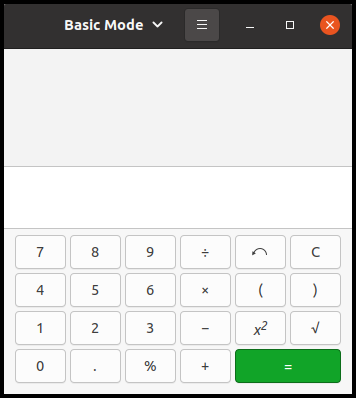
\includegraphics[width=5.34cm,height=5.97cm]{../image/gnome_calculator_basic.png}
\caption{gnome-calculator basic mode}
\end{figure}

Change the mode to advanced and quit.

\begin{figure}
\centering
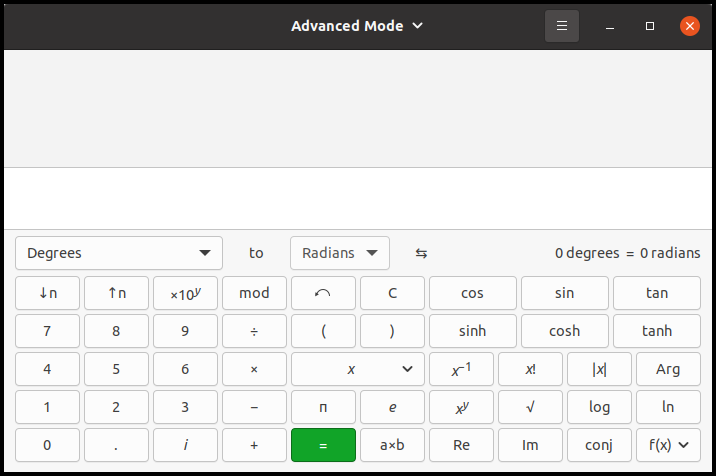
\includegraphics[width=10.74cm,height=7.14cm]{../image/gnome_calculator_advanced.png}
\caption{gnome-calculator advanced mode}
\end{figure}

Run gsettings and check the value of
\passthrough{\lstinline!button-mode!}.

\begin{lstlisting}
$ gsettings list-recursively org.gnome.calculator

... ...

org.gnome.calculator button-mode 'advanced'

... ...
\end{lstlisting}

Now we know that GNOME Calculator used gsettings and it has set
\passthrough{\lstinline!button-mode!} key to ``advanced''. The value
remains even the calculator quits. So when the calculator runs again, it
will appear as an advanced mode.

\subsubsection{Glib-compile-schemas
utility}\label{glib-compile-schemas-utility}

GSettings schemas are specified with an XML format. The XML schema files
must have the filename extension \passthrough{\lstinline!.gschema.xml!}.
The following is the XML schema file for the application
\passthrough{\lstinline!tfe!}.

\begin{lstlisting}[language=XML, numbers=left]
<?xml version="1.0" encoding="UTF-8"?>
<schemalist>
  <schema path="/com/github/ToshioCP/tfe/" id="com.github.ToshioCP.tfe">
    <key name="font-desc" type="s">
      <default>'Monospace 12'</default>
      <summary>Font</summary>
      <description>A font to be used for textview.</description>
    </key>
  </schema>
</schemalist>
\end{lstlisting}

The filename is ``com.github.ToshioCP.tfe.gschema.xml''. Schema XML
filenames are usually the schema id followed by ``.gschema.xml'' suffix.
You can use different name from schema id, but it is not recommended.

\begin{itemize}
\tightlist
\item
  2: The top level element is \passthrough{\lstinline!<schemalist>!}.
\item
  3: schema tag has \passthrough{\lstinline!path!} and
  \passthrough{\lstinline!id!} attributes. A path determines where the
  settings are stored in the conceptual global tree of settings. An id
  identifies the schema.
\item
  4: Key tag has two attributes. Name is the name of the key. Type is
  the type of the value of the key and it is a GVariant Format String.
\item
  5: default value of the key \passthrough{\lstinline!font-desc!} is
  \passthrough{\lstinline!Monospace 12!}.
\item
  6: Summery and description elements describes the key. They are
  optional, but it is recommended to add them in the XML file.
\end{itemize}

The XML file is compiled by glib-compile-schemas. When compiling,
\passthrough{\lstinline!glib-compile-schemas!} compiles all the XML
files which have ``.gschema.xml'' file extension in the directory given
as an argument. It converts the XML file into a binary file
\passthrough{\lstinline!gschemas.compiled!}. Suppose the XML file above
is under \passthrough{\lstinline!tfe6!} directory.

\begin{lstlisting}
$ glib-compile-schemas tfe6
\end{lstlisting}

Then, \passthrough{\lstinline!gschemas.compiled!} is generated under
\passthrough{\lstinline!tfe6!}. When you test your application, set
\passthrough{\lstinline!GSETTINGS\_SCHEMA\_DIR!} environment variable so
that GSettings objet can find
\passthrough{\lstinline!gschemas.compiled!}.

\begin{lstlisting}
$ GSETTINGS_SCHEMA_DIR=(the directory gschemas.compiled is located):$GSETTINGS_SCHEMA_DIR (your application name)
\end{lstlisting}

GSettings object looks for this file by the following process.

\begin{itemize}
\tightlist
\item
  It searches \passthrough{\lstinline!glib-2.0/schemas!} subdirectories
  of all the directories specified in the environment variable
  \passthrough{\lstinline!XDG\_DATA\_DIRS!}. Common directores are
  \passthrough{\lstinline!/usr/share/glib-2.0/schemas!} and
  \passthrough{\lstinline!/usr/local/share/glib-2.0/schemas!}.
\item
  If \passthrough{\lstinline!$HOME/.local/share/glib-2.0/schemas!}
  exists, it is also searched.
\item
  If \passthrough{\lstinline!GSETTINGS\_SCHEMA\_DIR!} environment
  variable is defined, it searches all the directories specified in the
  variable. \passthrough{\lstinline!GSETTINGS\_SCHEMA\_DIR!} can specify
  multiple directories delimited by colon (:).
\end{itemize}

The directories above includes more than one
\passthrough{\lstinline!.gschema.xml!} file. Therefore, when you install
your application, follow the instruction below to install your schemas.

\begin{enumerate}
\def\labelenumi{\arabic{enumi}.}
\tightlist
\item
  Make \passthrough{\lstinline!.gschema.xml!} file.
\item
  Copy it to one of the directories above. For example,
  \passthrough{\lstinline!$HOME/.local/share/glib-2.0/schemas!}.
\item
  Run \passthrough{\lstinline!glib-compile-schemas!} on the directory.
  It compiles all the schema files in the directory and creates or
  updates the database file \passthrough{\lstinline!gschemas.compiled!}.
\end{enumerate}

\subsubsection{GSettings object and
binding}\label{gsettings-object-and-binding}

Now, we go on to the next topic, how to program GSettings.

You need to compile your schema file in advance.

Suppose id, key, class name and a property name are:

\begin{itemize}
\tightlist
\item
  GSettings id: com.github.ToshioCP.sample
\item
  GSettings key: sample\_key
\item
  The class name: Sample
\item
  The property to bind: sample\_property
\end{itemize}

The example below uses \passthrough{\lstinline!g\_settings\_bind!}. If
you use it, GSettings key and instance property must have the same the
type. In the example, it is assumed that the type of ``sample\_key'' and
``sample\_property'' are the same.

\begin{lstlisting}[language=C]
GSettings *settings;
Sample *sample_object;

settings = g_settings_new ("com.github.ToshioCP.sample");
sample_object = sample_new ();
g_settings_bind (settings, "sample_key", sample_object, "sample_property", G_SETTINGS_BIND_DEFAULT);
\end{lstlisting}

The function \passthrough{\lstinline!g\_settings\_bind!} binds the
GSettings value and the property of the instance. If the property value
is changed, the GSettings value is also changed, and vice versa. The two
values are always the same.

The function \passthrough{\lstinline!g\_settings\_bind!} is simple and
easy but it isn't always possible. The type of GSettings are restricted
to the type GVariant has. Some property types are out of GVariant. For
example, GtkFontDialogButton has ``font-desc'' property and its type is
PangoFontDescription. PangoFontDescription is a C structure and it is
wrapped in a boxed type GValue to store in the property. GVariant
doesn't support boxed type.

In that case, another function
\passthrough{\lstinline!g\_settings\_bind\_with\_mapping!} is used. It
binds GSettings GVariant value and object property via GValue with
mapping functions.

\begin{lstlisting}[language=C]
void
g_settings_bind_with_mapping (
  GSettings* settings,
  const gchar* key,
  GObject* object,
  const gchar* property,
  GSettingsBindFlags flags, // G_SETTINGS_BIND_DEFAULT is commonly used
  GSettingsBindGetMapping get_mapping, // GSettings => property, See the example below
  GSettingsBindSetMapping set_mapping, // property => GSettings, See the example below
  gpointer user_data, // NULL if unnecessary
  GDestroyNotify destroy //NULL if unnecessary
)
\end{lstlisting}

The mapping functions are defined like these:

\begin{lstlisting}[language=C]
gboolean
(* GSettingsBindGetMapping) (
  GValue* value,
  GVariant* variant,
  gpointer user_data
)

GVariant*
(* GSettingsBindSetMapping) (
  const GValue* value,
  const GVariantType* expected_type,
  gpointer user_data
)
\end{lstlisting}

The following codes are extracted from
\passthrough{\lstinline!tfepref.c!}.

\begin{lstlisting}[language=C, numbers=left]
static gboolean // GSettings => property
get_mapping (GValue* value, GVariant* variant, gpointer user_data) {
  const char *s = g_variant_get_string (variant, NULL);
  PangoFontDescription *font_desc = pango_font_description_from_string (s);
  g_value_take_boxed (value, font_desc);
  return TRUE;
}

static GVariant* // Property => GSettings
set_mapping (const GValue* value, const GVariantType* expected_type, gpointer user_data) {
  char*font_desc_string = pango_font_description_to_string (g_value_get_boxed (value));
  return g_variant_new_take_string (font_desc_string);
}

static void
tfe_pref_init (TfePref *pref) {
  gtk_widget_init_template (GTK_WIDGET (pref));
  pref->settings = g_settings_new ("com.github.ToshioCP.tfe");
  g_settings_bind_with_mapping (pref->settings, "font-desc", pref->font_dialog_btn, "font-desc", G_SETTINGS_BIND_DEFAULT,
      get_mapping, set_mapping, NULL, NULL);
}
\end{lstlisting}

\begin{itemize}
\tightlist
\item
  15-21: This function \passthrough{\lstinline!tfe\_pref\_init!}
  initializes the new TfePref instance.
\item
  18: Creates a new GSettings instance. The id is
  ``com.github.ToshioCP.tfe''.
\item
  19-20: Binds the GSettings ``font-desc'' and the GtkFontDialogButton
  property ``font-desc''. The mapping functions are
  \passthrough{\lstinline!get\_mapping!} and
  \passthrough{\lstinline!set\_mapping!}.
\item
  1-7: The mapping function from GSettings to the property. The first
  argument \passthrough{\lstinline!value!} is a GValue to be stored in
  the property. The second argument \passthrough{\lstinline!variant!} is
  a GVarinat structure that comes from the GSettings value.
\item
  3: Retrieves a string from the GVariant structure.
\item
  4: Build a PangoFontDescription structure from the string and assigns
  its address to \passthrough{\lstinline!font\_desc!}.
\item
  5: Puts \passthrough{\lstinline!font\_desc!} into the GValue
  \passthrough{\lstinline!value!}. The ownership of
  \passthrough{\lstinline!font\_desc!} moves to
  \passthrough{\lstinline!value!}.
\item
  6: Returns TRUE that means the mapping succeeds.
\item
  9-13: The mapping function from the property to GSettings. The first
  argument \passthrough{\lstinline!value!} holds the property data. The
  second argument \passthrough{\lstinline!expected\_type!} is the type
  of GVariant that the GSettings value has. It isn't used in this
  function.
\item
  11: Gets the PangoFontDescription structure from
  \passthrough{\lstinline!value!} and converts it to string.
\item
  12: The string is inserted to a GVariant structure. The ownership of
  the string \passthrough{\lstinline!font\_desc\_string!} moves to the
  returned value.
\end{itemize}

\subsection{C file}\label{c-file}

The following is the full codes of \passthrough{\lstinline!tfepref.c!}

\begin{lstlisting}[language=C, numbers=left]
#include <gtk/gtk.h>
#include "tfepref.h"

struct _TfePref
{
  GtkWindow parent;
  GSettings *settings;
  GtkFontDialogButton *font_dialog_btn;
};

G_DEFINE_FINAL_TYPE (TfePref, tfe_pref, GTK_TYPE_WINDOW);

static void
tfe_pref_dispose (GObject *gobject) {
  TfePref *pref = TFE_PREF (gobject);

  /* GSetting bindings are automatically removed when the object is finalized, so it isn't necessary to unbind them explicitly.*/
  g_clear_object (&pref->settings);
  gtk_widget_dispose_template (GTK_WIDGET (pref), TFE_TYPE_PREF);
  G_OBJECT_CLASS (tfe_pref_parent_class)->dispose (gobject);
}

/* ---------- get_mapping/set_mapping ---------- */
static gboolean // GSettings => property
get_mapping (GValue* value, GVariant* variant, gpointer user_data) {
  const char *s = g_variant_get_string (variant, NULL);
  PangoFontDescription *font_desc = pango_font_description_from_string (s);
  g_value_take_boxed (value, font_desc);
  return TRUE;
}

static GVariant* // Property => GSettings
set_mapping (const GValue* value, const GVariantType* expected_type, gpointer user_data) {
  char*font_desc_string = pango_font_description_to_string (g_value_get_boxed (value));
  return g_variant_new_take_string (font_desc_string);
}

static void
tfe_pref_init (TfePref *pref) {
  gtk_widget_init_template (GTK_WIDGET (pref));
  pref->settings = g_settings_new ("com.github.ToshioCP.tfe");
  g_settings_bind_with_mapping (pref->settings, "font-desc", pref->font_dialog_btn, "font-desc", G_SETTINGS_BIND_DEFAULT,
      get_mapping, set_mapping, NULL, NULL);
}

static void
tfe_pref_class_init (TfePrefClass *class) {
  G_OBJECT_CLASS (class)->dispose = tfe_pref_dispose;
  gtk_widget_class_set_template_from_resource (GTK_WIDGET_CLASS (class), "/com/github/ToshioCP/tfe/tfepref.ui");
  gtk_widget_class_bind_template_child (GTK_WIDGET_CLASS (class), TfePref, font_dialog_btn);
}

GtkWidget *
tfe_pref_new (void) {
  return GTK_WIDGET (g_object_new (TFE_TYPE_PREF, NULL));
}
\end{lstlisting}

\subsection{Test program}\label{test-program}

There's a test program located at
\passthrough{\lstinline!src/tfe6/test!} directory.

\begin{lstlisting}[language=C, numbers=left]
#include <gtk/gtk.h>
#include "../tfepref.h"

GSettings *settings;

// "changed::font-desc" signal handler
static void
changed_font_desc_cb (GSettings *settings, char *key, gpointer user_data) {
  char *s;
  s = g_settings_get_string (settings, key);
  g_print ("%s\n", s);
  g_free (s);
}

static void
app_shutdown (GApplication *application) {
  g_object_unref (settings);
}

static void
app_activate (GApplication *application) {
  GtkWidget *pref = tfe_pref_new ();

  gtk_window_set_application (GTK_WINDOW (pref), GTK_APPLICATION (application));
  gtk_window_present (GTK_WINDOW (pref));
}

static void
app_startup (GApplication *application) {
  settings = g_settings_new ("com.github.ToshioCP.tfe");
  g_signal_connect (settings, "changed::font-desc", G_CALLBACK (changed_font_desc_cb), NULL);
  g_print ("%s\n", "Change the font with the font button. Then the new font will be printed out.\n");
}

#define APPLICATION_ID "com.github.ToshioCP.test_tfe_pref"

int
main (int argc, char **argv) {
  GtkApplication *app;
  int stat;

  app = gtk_application_new (APPLICATION_ID, G_APPLICATION_DEFAULT_FLAGS);
  g_signal_connect (app, "startup", G_CALLBACK (app_startup), NULL);
  g_signal_connect (app, "activate", G_CALLBACK (app_activate), NULL);
  g_signal_connect (app, "shutdown", G_CALLBACK (app_shutdown), NULL);
  stat =g_application_run (G_APPLICATION (app), argc, argv);
  g_object_unref (app);
  return stat;
}
\end{lstlisting}

This program sets its active window to TfePref instance, which is a
child object of GtkWindow.

It sets the ``changed::font-desc'' signal handler in the startup
function. The process from the user's font selection to the handler is:

\begin{itemize}
\tightlist
\item
  The user clicked on the GtkFontDialogButton and GtkFontDialog appears.
\item
  He/she selects a new font.
\item
  The ``font-desc'' property of the GtkFontDialogButton instance is
  changed.
\item
  The value of ``font-desc'' key on the GSettings database is changed
  since it is bound to the property.
\item
  The ``changed::font-desc'' signal on the GSettings instance is
  emitted.
\item
  The handler is called.
\end{itemize}

The program building is divided into four steps.

\begin{itemize}
\tightlist
\item
  Compile the schema file
\item
  Compile the XML file to a resource (C source file)
\item
  Compile the C files
\item
  Run the executable file
\end{itemize}

Commands are shown in the next four sub-subsections. You don't need to
try them. The final sub-subsection shows the meson-ninja way, which is
the easiest.

\subsubsection{Compile the schema file}\label{compile-the-schema-file}

\begin{lstlisting}
$ cd src/tef6/test
$ cp ../com.github.ToshioCP.tfe.gschema.xml com.github.ToshioCP.tfe.gschema.xml
$ glib-compile-schemas .
\end{lstlisting}

Be careful. The commands \passthrough{\lstinline!glib-compile-schemas!}
has an argument ``.'', which means the current directory. This results
in creating \passthrough{\lstinline!gschemas.compiled!} file.

\subsubsection{Compile the XML file}\label{compile-the-xml-file}

\begin{lstlisting}
$ glib-compile-resources --sourcedir=.. --generate-source --target=resource.c ../tfe.gresource.xml
\end{lstlisting}

\subsubsection{Compile the C file}\label{compile-the-c-file}

\begin{lstlisting}
$ gcc `pkg-config --cflags gtk4` test_pref.c ../tfepref.c resource.c `pkg-config --libs gtk4`
\end{lstlisting}

\subsubsection{Run the executable file}\label{run-the-executable-file}

\begin{lstlisting}
$ GSETTINGS_SCHEMA_DIR=. ./a.out

Jamrul Italic Semi-Expanded 12 # <= select Jamrul Italic 12
Monospace 12 #<= select Monospace Regular 12
\end{lstlisting}

\subsubsection{Meson-ninja way}\label{meson-ninja-way}

Meson wraps up the commands above. Create the following text and save it
to \passthrough{\lstinline!meson.build!}.

Note: Gtk4-tutorial repository has meson.build file that defines several
tests. So you can try it instead of the following text.

\begin{lstlisting}
project('tfe_pref_test', 'c')

gtkdep = dependency('gtk4')

gnome=import('gnome')
resources = gnome.compile_resources('resources','../tfe.gresource.xml', source_dir: '..')
gnome.compile_schemas(build_by_default: true, depend_files: 'com.github.ToshioCP.tfe.gschema.xml')

executable('test_pref', ['test_pref.c', '../tfepref.c'], resources, dependencies: gtkdep, export_dynamic: true, install: false)
\end{lstlisting}

\begin{itemize}
\tightlist
\item
  Project name is `tfe\_pref\_test' and it is written in C language.
\item
  It depends on GTK4 library.
\item
  It uses GNOME module. Modules are prepared by Meson.
\item
  GNOME module has \passthrough{\lstinline!compile\_resources!} method.
  When you call this method, you need the prefix ``gnome.''.

  \begin{itemize}
  \tightlist
  \item
    The target filename is resources.
  \item
    The definition XML file is `../tfe.gresource.xml'.
  \item
    The source dir is `..'. All the ui files are located there.
  \end{itemize}
\item
  GNOME module has \passthrough{\lstinline!compile\_schemas!} method. It
  compiles the schema file `com.github.ToshioCP.tfe.gschema.xml'. You
  need to copy `../com.github.ToshioCP.tfe.gschema.xml' to the current
  directory in advance.
\item
  It creates an executable file `test\_pref'. The source files are
  `test\_pref.c', `../tfepref.c' and
  \passthrough{\lstinline!resources!}, which is made by
  \passthrough{\lstinline!gnome.compile\_resources!}. It depends on
  \passthrough{\lstinline!gtkdep!}, which is GTK4 library. The symbols
  are exported and no installation support.
\end{itemize}

Type like this to build and test the program.

\begin{lstlisting}
$ cd src/tef6/test
$ cp ../com.github.ToshioCP.tfe.gschema.xml com.github.ToshioCP.tfe.gschema.xml
$ meson setup _build
$ ninja -C _build
$ GSETTINGS_SCHEMA_DIR=_build _build/test_pref
\end{lstlisting}

A window appears and you can choose a font via GtkFontDialog. If you
select a new font, the font string is output through the standard
output.
